\section{Agile Development}\label{sec:jira_ticket}

LSST data management follows a form of cyclic development often referred to as {\emph Agile} methodology. It is also beholden to organizations such as NSF which require a more traditional approach to project development such as the Earned Value Management System (EVMS).
We have presented this from both  the ESA and LSST perspective in SPIE previously  \cite{2014SPIE.9150E..1EG}.
In 2016  we presented a more complete approach for LSST to the problem of Agile in the earned value world \cite{2016SPIE.9911E..0NK}, here we provide just a brief update on that paper concentrating more on the Agile aspects.


\subsection{Management}
\cite{DMTN-020} provides a guide to the mechanisms underpinning LSST Data Management’s approach to project management, the reader is referred to to this for gory details as required.
Each institution in the DM team is still typically
responsible for 1 or more Level 2 WBS elements, and each institution has a Technical/Control Account Manager
(T/CAM) responsible for planning, estimating, monitoring and EVM reporting for that Level 2 WBS element.
The detailed management plan is in \cite{LDM-294}.

\subsection{Basic Assumptions}
The Project assumes that a full-time individual works for a total of
1,800 hours per year: this figure is \emph{after} all vacations, sick
leave, etc are taken into account. Staff appointed to ``developer''
positions are expected to devote this effort directly to LSST.

Appointment as a ``scientist'' includes a 20\% personal research time
allowance. That is, scientists are expected to devote 1,440 hours per
year to LSST, and the remainder of their time to personal research.

Our base assumption is that 30\% of an individual's LSST time (i.e. 540 hours/year for a developer, 432 hours/year for a scientist) are devoted to overhead for regular meetings\footnote{``Meetings'' include, for example, scheduled weekly team meetings, stand-ups, etc; major conferences or project meetings involving preparation, travel time, etc should be scheduled in advance and allocated Story Points}, ad-hoc discussions and other interruptions.
This is similar to the standard {\emph Agile} discount, however in the earned value world that must be accounted for and it is considered Level of Effort (LOE)


\section{Long Term Planning}
\label{sec:long-term-plan}

The plan for the duration of construction is embodied in:

\begin{enumerate}
\item
  A series of \emph{planning packages}, which describe major pieces of
  technical work. Planning packages are associated with concrete, albeit
  high-level, deliverables (in the shape of milestones), and have
  specific resource loads (staff assignments), start dates, and
  durations. The entire DM system is covered by around 100 of these
  planning packages.
\item
  \emph{Milestones} represent the delivery or availability of specific
  functionality. Each planning package culminates in a milestone, and
  may contain other milestones describing intermediate results.
\end{enumerate}

Planning packages are defined at the fourth level of the Work Breakdown Structure (WBS).

All WBS elements are related to the set of Data Management Products embodied in \citep{LDM-148} a high level summary of which is given in
Figure \ref{fig:prods}. Each product has a product owner to guide the agile development, this is frequently one of the Data Management Scientists.

\begin{figure}[htbp]
        \begin{center}
                 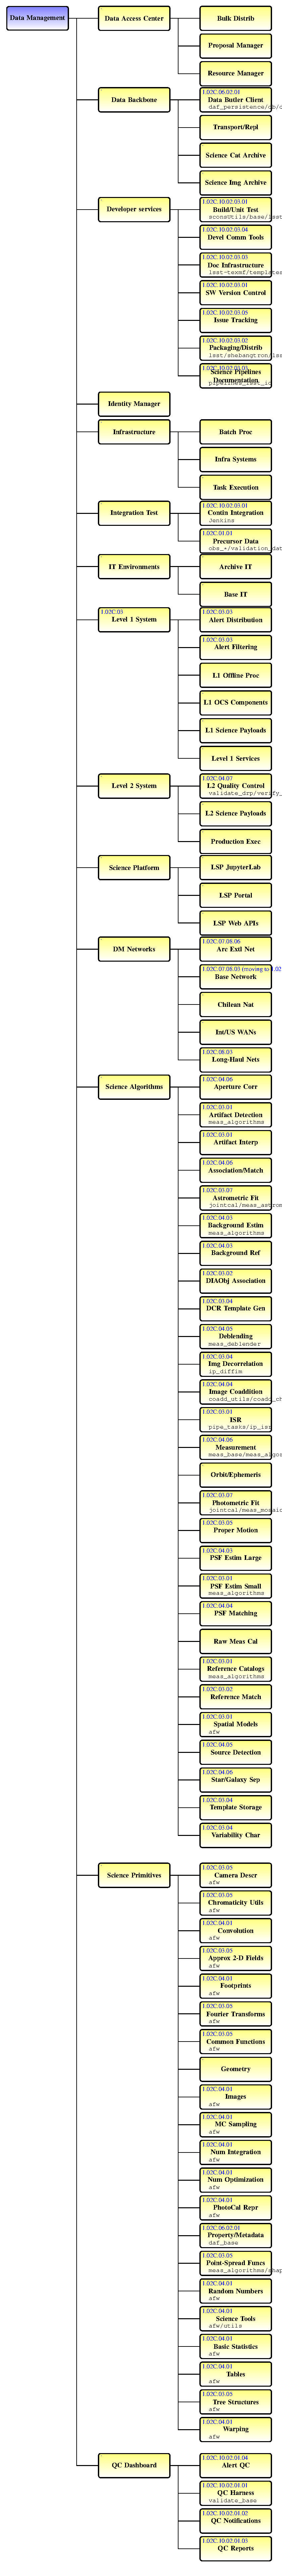
\includegraphics[height=19cm]{ProductTree}
                 \caption{DM product tree. \label{fig:prods}- there are over 200 products, this tree is to convey and idea of the products and is truncated to make it somewhat legible.
         }

         \end{center}
 \end{figure}

During the cycle planning process  effort is drawn from the budget embodied in the planning packages to generate the cycle plan, described in terms of epics in Jira.
Each epic itself has a particular budget.
This budget is subtracted from that available in the planning package at the point when the epic is defined.
Team members then add specific stories to these epics.

The Jira system is synchronized with the Primavera project management tool every three months using in house tools.

In order for the DM system to reach its science goals, new algorithmic or engineering approaches must sometimes be researched.
It is appropriate to budget time for this research work in planning packages.
Areas where successful delivery of the DM system is dependent on speculative research are a source of risk: where possible, the plan  also provides for a fallback option to be taken when research objectives are not achieved.
This may also lead to an entry in the risk register.



\section{Reporting }
Though the EVMS system is reasonable good for reporting it does not report well on Agile progress. Since  \citep{2016SPIE.9911E..0NK} we have undertaken a set of test driven milestones to show progress in Data Management.

Epics, stories, P6, milestones, EVMS.
How do we use product owners?
Test specifications and requirements.

How has this evolved since Kantor et al SPIE 2016? (kind of important that we link this SPIE paper to previous SPIE paper on Agile process).

